\section{S3 -- Metody tworzenia harmonogramów w projekcie informatycznym}
Obecnie istnieje wiele metodyk pozwalających na efektywne zarządzanie projektem, nie można jednoznacznie wybrać najlepszej, każda ma charakterystyczne elementy. Projekt można podzielić na etapy, określić przewidywany czas realizacji, zasoby, zależności między etapami.

Stosowaną np. przez Nas na seminarium dyplomowym metodą do określenia stanu zaawansowania prac nad naszą pracą inżynierską był wykres Gantta.

\textbf{Wykres Gantta} jest graficznym sposobem planowania i kontroli. Planowanie i koordynowanie przebiegu różnych czynności w przekroju czasowym odgrywa istotną rolę w tworzeniu i funkcjonowaniu organizacji. Wykresy Gantta służą do planowania działań wielopodmiotowych zarówno zespołowych, jak i grupowych. Przedstawiają następstwo kolejnych zdarzeń, uwzględniając również zadania wykonywane równolegle. Dzięki tej technice można także kontrolować realizację zaplanowanego przedsięwzięcia.

Podstawowym celem jest wspomaganie pracy kierownika projektu dzięki podkreślaniu związków między zadaniami oraz wpływu potencjalnych zmian na cały projekt. Pozwala również przeprowadzać symulację, która umożliwia określenie proponowanych zmian na specyfikację, dostępność zasobów i ustalone terminy. Wykres Gantta pełni także zasadniczą rolę w czasie optymalizowania pierwszej ,,realistycznej” wersji planu projektu.

\begin{figure}[H]
	\centering
	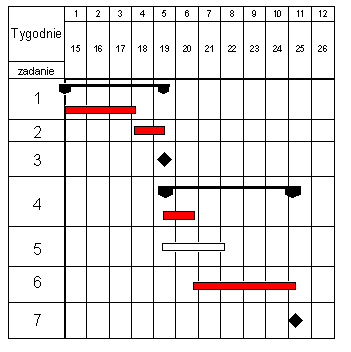
\includegraphics[scale=0.7]{s3_gantt.png}
	\caption{Przykładowy wykres Gantta z zadaniami krytycznymi, niekrytycznymi, kamieniami milowymi i podsuowaniami}
\end{figure}

Oprócz tego sposób organizacji czasu wyznaczają metodyki stosowane w projekcie informatycznym:

\begin{itemize}
	\setlength\itemsep{1pt}
	\item \textbf{Model kaskadowy} - projekt jest dzielony na sześć do ośmiu faz, które następują kolejno po sobie. Danymi wejściowymi dla każdej fazy są dane wyjściowe fazy poprzedniej. Model stosowany jest w projektach o dobrze zdefiniowanych wymaganiach, stosowany najczęściej w projektach małych.
	
	\begin{figure}[H]
		\centering
		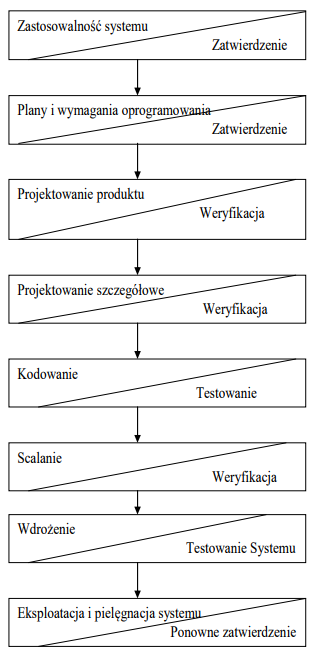
\includegraphics[scale=0.6]{s3_kaskadowy.PNG}
		\caption{Przykładowy proces kaskadowy}
	\end{figure}
	
	\begin{itemize}
		\setlength\itemsep{1pt}
		\item[] \textbf{Zalety metody:}
		\item Cały proces jest dobrze udokumentowany i ustalony z klientem.
		\item Ułatwia organizację: planowanie, harmonogramowanie i monitorowanie projektu
		\item Wszystkie wymagania są analizowane i zatwierdzane przez klienta, klient sam może oszacować korzyści z wdrożenia systemu
		\item Wymusza dokończenie dokumentacji po każdej fazie
	\end{itemize}
	
	\begin{itemize}
		\setlength\itemsep{1pt}
		\item[] \textbf{Wady:}
		\item Ścisła kolejność wykonywanych prac – realizatorzy poszczególnych faz nie mogą pracować równolegle
		\item Mała możliwość modyfikacji projektu
		\item Wysokie koszty błędów popełnionych we wczesnych fazach
		\item Testowanie systemu dopiero po zakończeniu programowania – może powodować poprawianie „na skróty”
		\item Niedopasowanie do rzeczywistości – rzeczywiste projekty rzadko są sekwencyjne
	\end{itemize}
	
	\item \textbf{Model spiralny} - rozwinięcie metody kaskadowej – polecany w przypadku dużych, drogich i skomplikowanych projektów. Istota sprowadza się do tego, że jest to iteracyjna metoda kaskadowa.
	
	\begin{figure}[H]
		\centering
		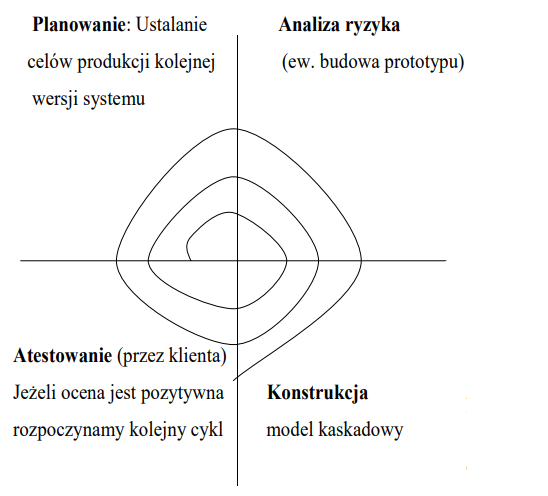
\includegraphics[scale=0.6]{s3_spiralny.PNG}
		\caption{Przykładowy proces spiralny}
	\end{figure}
	
	\begin{itemize}
		\setlength\itemsep{1pt}
		\item[] \textbf{Zalety metody:}
		\item Cały system powstaje we współpracy z klientem
		\item Wszystkie braki fazy ustalania wymagań są identyfikowane w miarę postępu prac
	\end{itemize}
	
	\begin{itemize}
		\setlength\itemsep{1pt}
		\item[] \textbf{Wady:}
		\item Wymagana jest dyscyplina po stronie klienta
		\item Kontrola wykonawcza jest trudna, bo klient nie odpowiada ani za budżet ani za harmonogram
	\end{itemize}
	
	\item \textbf{SCRUM} jest metodyką adaptacyjną, która w szybkim tempie zyskuje popularność na całym świecie - również w Polsce. Jako jeden z powodów sukcesu SCRUM podaję się fakt, iż daje on konkretny i spójny przepis na prowadzenie projektów informatycznych oferując przy tym dużą swobodę jeśli chodzi o sposób implementacji w konkretnej organizacji
	
	SCRUM definiuje cztery główne role w projekcie:
	\begin{itemize}
		\setlength\itemsep{1pt}
		\item Właściciel produktu – jest to klient lub sponsor projektu odpowiedzialny za kwestie biznesowe
		\item ScrumMaster - jest to osoba odpowiedzialna za kontrolę przebiegu procesów
		\item Członek zespołu - osoba należąca do zespołu realizującego projekt bez względu na wykonywane czynności. (programista, analityk etc.)
		\item Interesariusze – osoby odpowiedzialne za podejmowanie decyzji strategicznych, których taktyczną implementację prowadzi właściciel produktu. Interesanci nie biorą czynnego udziału w codziennych spotkaniach zespołu projektowego – mogą jednak pełnić rolę obserwatorów.
	\end{itemize}
	
	Zespół projektowy pracuje w określonym przedziale czasowym zwanym przebiegiem (ang. \textbf{sprint}). Efektem przebiegu za każdym razem powinno być dostarczenie użytkownikom kolejnego działającego produktu. Zasadą jest to, że zmiany wprowadzane w jednym przebiegu muszą być namacalne dla użytkowników. Muszą wnosić wartość funkcjonalną. Przebieg może trwać \textbf{od 2 do 6 tygodni}. Zaleca się stosowanie przebiegów o stałych długościach.
	
	W pierwszym etapie tworzona jest lista wymagań użytkownika, są one gromadzone w postaci \textbf{"historyjek"}. Każda historyjka opisuje jedną cechę systemu. Właściciel projektu jest też zobowiązany do przedstawienia priorytetów wymagań oraz głównego celu przebiegu. Po tym formułowany jest rejestr wymagań. Cel przebiegu jest \textbf{zapisywany w widocznym miejscu} w pokoju członków zespołu.
	
	Następnie wybierane są zadania o najwyższym priorytecie, a jednocześnie przyczyniające się do realizacji celu projektu. Szacuje się czas realizacji każdego zadania. Lista zadań wraz z oszacowaną czasochłonnością nosi nazwę rejestru zadań przebiegu (\textbf{sprint backlog}).
\end{itemize}